\documentclass{beamer} 
\usetheme{default}
\usecolortheme{albatross} 
\setbeamercovered{transparent}

%\useoutertheme{umbcfootline} 
%\setbeamertemplate{background canvas}[vertical shading][bottom=red!20,top=yellow!30] 


\usepackage[spanish]{babel}
%\usepackage[latin1]{inputenc}
\usepackage[utf8x]{inputenc}



\title{POO}

\author{Manuel J. Molino Milla \and Luis Molina Garzón}

\date{\today} %

\institute{IES Virgen del Carmen \and Departamento de Informática}




%\beamerdefaultoverlayspecification{<+->}

\begin{document}


\begin{frame}
  \titlepage
\end{frame}

\begin{frame}
    \frametitle{Logo}
\begin{figure}

\includegraphics[scale=1]{imagenes/logo.jpeg} 
\caption{Logo Java}
\end{figure}
\end{frame}

\begin{frame}
  \frametitle{Contenido}
  \tableofcontents[pausesections]
\end{frame}



\section{Introduccion}

\subsection{Introduccion}
\begin{frame}
\frametitle{¿Que es un objeto?}
\begin{itemize}[<+->]
\item Un objeto representa una entidad en el mundo real que se puede identificar claramente.
\item Por ejemplo, un estudiante, un escritorio, un círculo, un botón, e incluso un préstamo todos pueden ser vistos como objetos.
\item Un objeto tiene una identidad única definido por su estado y su comportamiento.
\begin{description}
\item[Estado] También conocido como sus propiedades o atributos. Ejemplo para un círculo un atributo puede ser el radio. Un rectángulo su ancho y alto.
\item[Comportamiento] También conocido como sus acciones y es definida por \emph{métodos}. Cuando invocamos un método le estamos pidiendo al objeto que haga algo. Ejemplo \emph{getArea()} en un círculo nos daría el área. 
\end{description}
\end{itemize}
\pause
\end{frame}

\begin{frame}
\frametitle{Objetos}
\begin{itemize}[<+->]
\item Objetos de un mismo tipo son definidos usando una clase común.
\item Una \emph{clase} es una plantilla o modelo que nos dice que atributos y métodos tendrá un objeto.
\item Un objeto es una \emph{instancia} de una clase.
\item Podemos crear muchas \emph{instancias} de una clase.
\item Los términos \emph{objetos} e \emph{instancias} son sinónimos.
\item La relación entre las clases y los objetos es análoga a la que existe entre una receta de pastel de manzana y pastel de manzana.
\item Podemos hacer tantas tartas de manzana como quieras de una sola receta
\end{itemize}
\pause
\end{frame}


\subsection{Diagramas UML}
\begin{frame}
\frametitle{Clase círculo} 
\begin{figure}
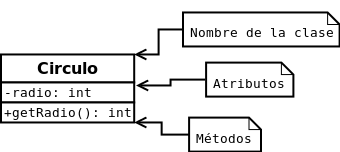
\includegraphics[scale=0.9]{imagenes/circulo.png} 
\caption{UML de la clase círculo}
\end{figure} 
\end{frame}

\begin{frame}
\frametitle{Clase rectángulo} 
\begin{figure}
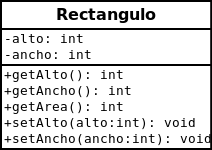
\includegraphics[scale=0.9]{imagenes/rectangulo.png} 
\caption{UML de la clase rectangulo}
\end{figure} 
\pause
\begin{itemize}
\item El signo \textbf{+} indica que el atributo o método es de acceso público.
\item El signo \textbf{-} indica que el atributo o método es de acceso privado.
\end{itemize}
\pause
\end{frame}

\begin{frame}
    \frametitle{Introduccion}

\begin{itemize}[<+-| alert@+>]
      \item Java es un lenguaje orientado a objetos \emph{puros}
      \item C++ y Java es un lenguaje hibrido.
      \item En Java se asume que se desea realizar \emph{POO}      
      \item Todo \emph{objeto} se manipula mediante \emph{referencias}.
      \item Simil: una television (objeto) se manipula con un mando a distancia (la referencia).
      \item Todos los objetos se crean usando la palabra clave \bf{new}
      \item Las referencias se almacenan en la pila.
      \item Los objetos se almacenan en el monticulo.
      \item Hemos visto que existen los tipos de datos \emph{primitivos}
      \item Los objetos los podemos considerar nuevos tipos de datos.
    \end{itemize}
    \pause
\end{frame}

\section{Clases}
\subsection{Introduccion}

\begin{frame}[fragile]
    \frametitle{Tipos de datos}
      En otros lenguajes se suele usar palabras claves. Ejemplo C: \\
    \begin{center}
    
     \begin{tiny}
 \begin{verbatim}
typedef enum enumCargo {
   programador,
   analista,
   analistafuncional,
   directorproyecto,
   stakeholder
} cargo;

typedef struct structEmpleado {
    int salario;
    cargo funcion;
} empleado;

typedef struct structAutonomo {
   int coste_horas_trabajador;
   int horas_dedicacion;
   cargo funcion;
} autonomo;

typedef union unionParticipante {
    empleado trabajador;
    autonomo jefe;
} participante;
\end{verbatim}
\end{tiny}
\end{center}
\end{frame}

\subsection{Definicion de clases}
\begin{frame}
    \frametitle{Clases}
    \framesubtitle{En Java utilizamos clases}

\begin{itemize}[<+-| alert@+>]

      \item Los lenguajes \emph{OO} suelen usar la palabra \bf{class}
      \item \emph{class UnNuevoTipo} \{código de la clase\}
      \item Creamos los nuevos tipos de esta manera:
      \item \emph{UnNuevoTipo t = new UnNuevoTipo();}
      \item Comparemos con los datos primitivos:
      \item int numeroEntero;
      \item double numeroReal = 2.23;
      \item No definimos ni \emph{int} o \emph{double} porque van implicitos en java.
      \item \emph{POO} conlleva la creacion de objetos y el envio de mensajes entre dichos objetos.
      \item Las clases definen los atributos de los objetos (caracteristicas).
      \item Y tambien los metodos usados para intercambiar mensajes entre los objestos.
\end{itemize}
\pause
\end{frame}

\subsection{Campos}


\begin{frame}[fragile]
    \frametitle{Campos}
    \framesubtitle{Son los atributos de los objetos}
\pause
\emph{Ejemplo de una clase Fecha:}\\
\begin{verbatim}
public class Fecha{
    private int dia;
    private int mes;
    private int anno;
}
\end{verbatim}   
\pause
\emph{Podemos usar la clase:} \\
\begin{verbatim}
public class TestFecha{
    public static void main(String[] args){
        Fecha f = new Fecha();
        f.dia=23;
        f.mes=12;
        f.anno=2001;}
    }
\end{verbatim}
\pause
Genera un error de compilacion: \emph{The field Fecha.dia is not visible} 
\end{frame}

\subsection{Métodos}

\begin{frame}[fragile]
    \frametitle{Métodos}
    \framesubtitle{Son lo que se conoce como funciones en programacion}
    \pause
  \begin{scriptsize}
  A traves de ellos podemos acceder a los atributos y darles valores. \emph{getters y setters}
  \pause
\begin{verbatim}
public class Fecha{
    private int dia;
    private int mes;
    private int anno;
}

public int getDia(){
    return dia;
}

public void setDia(int valor){
    dia=valor;
}
public int getMes(){
    return mes;
}

public void setMes(int valor){
    mes=valor;
}
public int getAnno(){
    return anno;
}

public void setAnno(int valor){
    anno=valor;
}
\end{verbatim}
\end{scriptsize}

\end{frame}

\begin{frame}
    \frametitle{Métodos}
    \begin{block}{Métodos de acceso}
\begin{itemize}[<+-| alert@+>]
\item Podemos acceder a los atributos a pesar \emph{private}.
\item Se llaman métodos de acceso ya que podemos obtener su valor \emph{get} o asignarle valor \emph{set}.
\item Al ser atributos privados solo se pueden acceder desde la clase.
\item Esto recibe el nombre de \emph{encapsulamiento}.
\end{itemize}
\end{block}
\pause
\end{frame}

\begin{frame}[fragile]
\frametitle{Ejemplo de uso de objetos}
\begin{verbatim}
public class TestFecha{
    public static void main(String[] args){
        Fecha f = new Fecha();
        f.setDia(23);
        f.setMes(12);
        f.setAnno(2001);
        System.out.println("Día: "+f.getDia());
        System.out.println("Mes: "+f.getMes());
        System.out.println("Año: "+f.getAnno());
     }
}
\end{verbatim}
\end{frame}

\begin{frame}
\frametitle{Crear y usar objetos}
\begin{block}{Pasos para crear y usar objetos}
\begin{itemize}[<+-| alert@+>]
\item Definimos el objeto, \emph{creamos una referencia en la pila}
\item Fecha f;
\item Creamos (instanciamos) el objeto, \emph{reservamos memoria en el monticulo}
\item f = new Fecha();
\item Las dos lineas anteriores se pueden crear en una sola:
\item Fecha f = new Fecha();
\item A partir de aqui usamos los \emph{setters} y \emph{getters}
\end{itemize}
\end{block}
\pause
\end{frame}




\begin{frame}[fragile]
    \frametitle{Otros metodos que no son de acceso}
 \begin{footnotesize}
   \begin{verbatim}
public class Numero{
    private int digito;
    public void setValor(int valor){
        digito=valor;
    }
    public int getValor(){
        return digito;
    }
    public int valorDoble(){
        return digito*2;
    }
}
\end{verbatim}
\pause
\begin{verbatim}
public class TestNumero{
    public static void main(String[] args){
        Numero n = new Numero();
        n.seValor(23);
        System.out.println("Numero: "+n.getValor());
        System.out.println("Doble: "+n.valorDoble());
     }
}
\end{verbatim} 
\end{footnotesize}  
\end{frame}

\subsection{Generalidades}
\begin{frame}
    \frametitle{Generalidades}
\begin{itemize}[<+->]
\item Las clases se suelen escribir en mayuscula.
\item Si la clase se llama \emph{Numero}
\item Se guarda en un fichero llamado \emph{Numero.java}
\item Hay metodos que retornan valores.
\item En este caso indicamos que tipo de valor:
\item public \emph{int} getValor()
\item Indicamos lo que se devuelve con \emph{return valor}
\item Cuando no se retorna ningun valor implica:
\item Se retorna el tipo \emph{void}
\item \emph{public \emph{void} setValor(int valor)} 
\item A veces hay que pasarle parámetros
\item Entre parentesis indica el parametro que se le pasa al metodo.
\item \emph{public void serValor(int valor)}
\end{itemize}
\pause
\end{frame}

\subsection{Parametros y valores de retorno}
\begin{frame}
\frametitle{Parametros y valores de retorno}
\begin{footnotesize}
\begin{block}{Definicion de metodo}
\begin{itemize}[<+->]
\item Las partes fundamentales de un metodo son:
\item \emph{Nombre}
\item \emph{Sus parametros}
\item \emph{Los valores de retorno}
\end{itemize}
\end{block}
\pause
\begin{block}{Metodo:}
\begin{itemize}[<+-|alert@+>]
\item tipoRetorno nombreMetodo ( /* Lista parametros*/ ) \{
\item /* Cuerpo del metodo */
\item \}
\end{itemize}
\end{block}
\pause
\begin{block}{Ejemplo:}
\begin{itemize}[<+-|alert@+>]
\item int sumaValores  (int valorUno, int ValorDos) \{
\item return valorUno+valorDos;
\item \}
\end{itemize}
\end{block}
\end{footnotesize}
\pause
\end{frame}

\begin{frame}
\frametitle{Métodos}
\begin{itemize}[<+->]
\item El tipo de retorno es el tipo de valor que surge después de invocarlo.
\item \emph{public int metodoNuevo(\dots} 
\item int numero = metodoNuevo(\dots
\item La lista de parámetros indica los tipos y nombres de la informaciones que es necesario pasar a ese método.
\item Cada método se identifica por el nombre del método y la lista de parámetros.
\item \emph{public int metodoUno( int Uno, int Dos) \{\dots}
\item \emph{public int metodoUno( int Uno) \{\dots}
\item \emph{public int metodoUno( double Uno) \{\dots}
\item \emph{public int metodoDos( double Uno) \{\dots}
\end{itemize}
\pause
\end{frame}

\begin{frame}
\frametitle{Lista de parámetros y return}
\begin{itemize}[<+-|alert@+>]
\item La lista de parámetros indica la informacion que se le pasa al metodo.
\item Se puede pasar tanto tipos primitivos como objetos o \emph{nada}
\item \emph{int metodo (int valor, Numero numero)\{\dots}
\item \emph{double metodoPI()\{\ return 3.1416;\}}
\item La palabra \emph{return} devuelve el valor y obliga a abandonar el metodo.
\item \emph{boolean indicador()\{\ return true;\}}
\item \emph{float naturalLogBase()\{\ return 2.718f;\}}
\item \emph{void nada()\{\ return;\}}
\item \emph{void nada2()\{\ \}}
\item En el caso de que el valor de retorno es \emph{void} es innecesario la palabra \emph{return}
\end{itemize}
\pause
\end{frame}

\begin{frame}[fragile]
\frametitle{Lista de parámetros dinamica}
Podemos hacer llamadas del mismo metodo con distinto numero de parametros, siempre que sean del mismo tipo:
\pause
\begin{verbatim}
public class Arg {

  public static void main(String[] args) {
    System.out.println("Suma: " + suma(1));
    System.out.println("Suma: " + suma(1,2));
    System.out.println("Suma: " + suma(1,2,3));
  }
  public static int suma (int ... args) {
    int suma = 0;
    for (int i = 0; i < args.length; i++)
      suma += args[i];
    return suma;
  }
}
\end{verbatim}
\end{frame}

\begin{frame}[fragile]
\frametitle{Javadoc: param y return}
\begin{footnotesize}
\begin{verbatim}
/**
 * Returns an Image object that can then be painted on the screen. 
 * The url argument must specify an absolute {@link URL}. The name
 * argument is a specifier that is relative to the url argument. 
 * <p>
 * This method always returns immediately, whether or not the 
 * image exists. When this applet attempts to draw the image on
 * the screen, the data will be loaded. The graphics primitives 
 * that draw the image will incrementally paint on the screen. 
 *
 * @param  url  an absolute URL giving the base location of the image
 * @param  name the location of the image, relative to the url argument
 * @return      the image at the specified URL
 * @see         Image
 */
 public Image getImage(URL url, String name) {
        try {
            return getImage(new URL(url, name));
        } catch (MalformedURLException e) {
            return null;
        }
 }
\end{verbatim}
\end{footnotesize}
\end{frame}


\subsection{Constructor}
\begin{frame}[fragile]
\frametitle{Constructor}
\begin{itemize}[<+-|alert@+>]
\item Permite inicializar objetos.
\item Si una clase tiene un constructor, \emph{Java} llama automaticamente a este metodo cuando se crea un objeto.
\item El nombre del constructor coindice con el nombre de la clase.
\item Ejemplo:
\begin{verbatim}
class Numeros {
    Numeros() {
        System.out.println("Creando numero");
    }
}    
public class Ejemplo {
    public static void main(String[] args){
        new Numeros();
    }
}    
\end{verbatim}
\item ¿Cómo se debe llamar al programa \emph{Numero.java} o \emph{Ejemplo.java}?
\item ¿Cuál es la salida de dicho programa?
\end{itemize}
\pause
\end{frame}

\begin{frame}[fragile]
\frametitle{Constructores}
\begin{itemize}[<+-|alert@+>]
\item Cuando se ejecuta \emph{new Numero()}:
\item Se asigna almacenamiento y se invoca al constructor.
\item A diferencia de otros metodos, suele escribirse en mayuscula.
\item Los constructores pueden tener parámetros.
\item Ejemplo:
\begin{verbatim}
class Numerosss {
    Numerosss(int valor) {
        System.out.println("Creando numero: "+valor);
    }
}    
public class Ejemplo1 {
    public static void main(String[] args){
        new Numeross(24);
    }
}    
\end{verbatim}
\item ¿Pueden tener valor de retorno los constructores?
\item No confudir con los \emph{setters}
\end{itemize}
\pause
\end{frame}

\begin{frame}[fragile]
\frametitle{Sobrecarga de métodos}
Permite crear un objeto de mas una manera
\pause
\begin{scriptsize}
\begin{verbatim}
class Numero1 {
        Numero1() {
                System.out.println("Creando numero");
        }
        Numero1(int valor) {
                System.out.println("Creando numero: "+valor);
        }
        Numero1(double valor) {
                System.out.println("Creando numero: "+valor);
        }
        Numero1(int valor1, int valor2) {
                System.out.println("Creando numero: "+valor1+valor2);
        }
}
public class Ejemplo2 {
        public static void main(String[] args){
                new Numero1();
                new Numero1(1);
                new Numero1(1.1);
                new Numero1(1,2);
        }
}
\end{verbatim}  
\end{scriptsize}  
\pause
¿Es correcto este programa? ¿Qué produce su salida?
\end{frame}


\begin{frame}[fragile]
\frametitle{Constructores}
\begin{itemize}[<+->]
\item ¿Como distingue \emph{Java} el constructor a invocar?
\item Por los parámetros.
\item Numero() Numero(int i) Numero(int i,int j) Numero(double i)
\item ¿Que ocurre en el siguiente código?
\begin{verbatim}
class Numero2{
    int i;
}

public class Ejemplo3{
    public static void main(String[] args){
    Numero2 n = new Numero2();
    }
}
\end{verbatim}
\item ¿Cómo se debe llamar el programa Numero.java o Ejemplo.java?
\item No tiene constructor. ¿Funciona?
\item El compilador de \emph{Java} crea uno automáticamente.
\end{itemize}
\end{frame}
\begin{frame}
\frametitle{Preguntas} 
\begin{figure}

\includegraphics[scale=0.9]{imagenes/dudas.png} 
\caption{Lenguaje máquina}
\end{figure} 
\end{frame}
\end{document}

